
\section{Texture in Scene Images}

In computer graphics, texture mapping is a powerful tool which adds the surface detail to an object by wrapping
the color information from a digitized image. 
Texture is applied on top of a
polygon or 3D model to obtain a realistic rendering of it.
This makes rendering of objects more realistic than those without
surface texture. 
Scene images are extensively
used as source of textures as they are able to capture visual and structural information of the real world. They
are also able to capture a high level detail of object properties.
Generally an image is used as a texture map
on a planar surface. 
%Image-based rendering techniques are widely used in computer graphics.
%Most frequently image-based rendering appears in the form of texture mapping 
%when an image is used to represent a complex object's 
%appearance. Texture mapping has several significant limitations, the primary one being that only a single lighting 
%condition is captured. If dynamic lighting is needed, texture mapping alone is insufficient. 

There are several texture mapping methods that avoids
modeling of the complex surface details. 
One of them is image-based rendering technique which is frequently used in computer graphics
in the form of texture mapping. The images are used to represent the appearance of a complex object.
It is a technique where images are used in place of complex geometry and material 
properties. Images are a quick way to achieve photorealism when our primary objective is to get 
a realistic rendering. This is because they are able to capture 
complex light interactions such as inter-reflections,
self-shadowing, and sub-surface scattering present in the real world.
The main disadvantage of using images as rendering source is that the image captures the
appearance of the object from a single viewpoint and under a fixed lighting condition/direction. 
Therefore this method fails if the lighting conditions of the synthetic
environment are different from the lighting conditions of the texture image. 
To solve this
problem, 
people have used techniques like Bump Mapping, Bidirectional
Reflectance Distribution Function (BRDF) and Polynomial texture maps. 
%First we will show how 2D and 3D texture differs from each other.
%Then we will describe the above mentioned techniques. 

\subsection{2D texture VS 3D texture}

In 2D texture modelling, the reflectance and the strutural properties of natural surfaces
are not captured. They fail to capture the variations in surfaces for different lighting and
viewing directions. The texture which is mapped onto a 3D model has
the lighting direction from which it was captured. So if we want to see how the texture looks from
different lighting direction, this mapping will give poor results when viewed from different
lighting direction apart from the direction from which it was captured. In general, real world objects
are not flat and smooth in nature. They show different types of structural variation across their
surface each having different reflectance properties. These properties causes effects like shadows,
specularity, sub-surface scattering, inter-reflection etc. Hence 3D texture mapping
is required for realisting modelling of real objects.
It results in realistic rendering
of natural material surfaces. The characterization of surface reflectance properties is important in
achieving enhanced realism of the scene. The appearance of a surface in different lighting and viewing direction/
conditions is affected by its reflectance properties.
3D textures are a way to model the relation between surface reflectance
properties and illumination/viewing conditions. Fig \ref{} shows the
3D texture mapped onto a 3D teapot model. Reflectance texture maps are one of
the techniques that can be used to compactly represent the 3D textures. These
maps are generated using image re-lighting techniques in which
multiple images are captured under different lighting/viewing conditions.


\begin{figure}[t]
\centering
\subfigure{
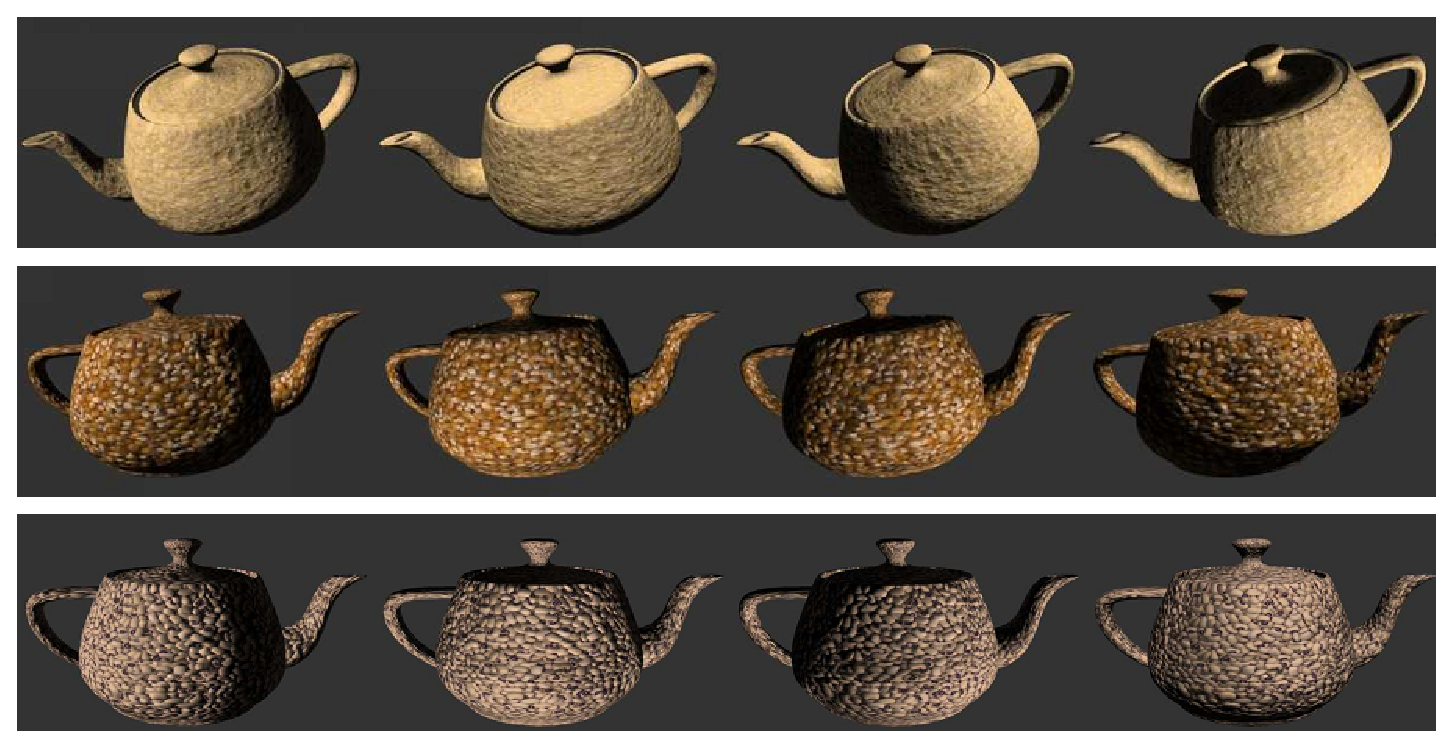
\includegraphics[height=4.2in,width=6in]{chap2/texture/res_1.eps}
}
\caption
{(a) Image containing Text over another Text (b) Foreground Text (c) Background Text (d)
Text extracted}
\end{figure}


\subsection{Bump Mapping}

Bump mapping, normal mapping, and other related techniques have been developed to extend texture mapping to
reproduce such light and view dependent dynamic effects. As with texture mapping, these methods store spatially
variant information for rendering. However, instead of storing a texture image that already contains some existing
illumination effects as in typical texture mapping, these methods store parameters that allow a computational 
lighting model to be varied spatially. Since these methods are often used with simple synthetic reflectance models
such as Phong lighting they achieve dynamic illumination at the expense of photorealism.
Bump maps and other similar methods typically use a map that has been generated by an artist or a procedural
method, rather than one captured from real world objects. Creating a bump map from photographs of real objects
is difficult, and is generally not done for games or other realistic renderings. Research techniques have been
developed to calculate bump maps automatically from multiple images of an object under known light directions 
[Rushmeier 97]. Unfortunately these methods typically have difficulty generating bump maps from objects that 
contain self-shadowing and intra-object interreflections. Even if methods could be derived that could generate
bump maps in the presence of such illumination effects, the resulting renderings would not recreate them properly
due to the limitations of these rendering techniques.

Bidirectional Reflectance Distribution Function, which defines the
spectral and reflectance characteristics of a surface can be used to create
reflectance texture maps. It is defined as the ratio of reflected radiance to
incident irradiance, given the lighting and viewing directions. The reflectance
at each point on a surface is hence a function of four parameters, controlling
the above two directions. Various techniques have been developed to compactly
represent BRDF. It was extended to Bidirectional
Texture Function by allowing BRDF to vary spatially across planar
texture co-ordinate (u,v).

.3D texture actually models the relation
between surface reflectance properties and illumination direction. They are represented
by Reflectance Texture Maps.These maps are generated using image re-lighting techniques
which model the surface reflectance properties of object.

%2D texture modelling fails to capture the surface variation and reflectance properties under
%varying lighting and viewing direction.They appear good only when viewed from similar lighting
%direction in which they were captured.2D textures appear flat and smooth but reflectance properties
%of real world objects are characterised by inter-reflections,shadows,specularity and sub-surface
%scattering. 2D texture fails to provide the information required for rendering other than the original
%illumination condition. Figure 1 illustrates how  the same texture behaves differently under different lighting conditions.

%It is clear from thefigure that 2D texture which has only the color information alone is not sufficient for a realisitic
% rendering of real world texture
%and therefore 3D texture is needed.

Reflectance map required in 3D texture can be modelled by Bidirectional Reflectance Distribution
Function \cite{B1} technique which defines spectral and spatial reflectance characteristic of a
surface.BRDF is the ratio of reflected radiance to incident irradiance.Various techniques have been
developed to compactly represent BRDF \cite{B5,B8,B12,B14,B15}.

BRDF was extended to Bidirectional Texture Function \cite{B2} by allowing BRDF to vary spatially
across planar texture co-ordinate (u,v)

(uncomment)
\begin{math}
$\[BTF=(\theta_{v},\phi_{v},\theta_{e},\phi_{e},u,v)\]$
\end{math}


BTF effectively captures view point dependent phenomenon such as specularity
along with other physical phenomenon such as shadow, sub-surface scattering,
inter-reflection, etc. However, the capture of BTF requires careful camera
calibration and capturing numerous images for sampling. Generating reflectance
map from BTF is very complex. View dependent appearances can also be modeled
using Light field maps. They offer a more compact representation and
can be used for a real time rendering of surface light fields.

Because of the  high dimensionality of the BTF and high storage requirement,
Unidirectional Texture Functions (UTF) were introduced in which viewing point is
not taken into account while modeling the surface reflectance properties. They
model these properties only in relation to different lighting conditions. As the
visual appearance of the surface is mostly independent of the viewing direction,
the model provides a reasonable approximation of the surface with significantly
lower complexity of the model.

Polynomial Texture Maps belong to the class of UTFs. It is a pixel
based technique that concisely models the surface reflectance properties using a
polynomial model for the reflectance, dependent on two angular parameters of the
lighting direction. PTMs reconstruct the color of the surface under varying
lighting conditions and models real world phenomenon such as
self-shadowing,inter-reflection and sub-surface scattering. They thus introduce
enhanced photorealism in the texture mapping process.

\subsection{Image Based Rendering}





Image-based methods yield photorealistic renderings that are based on
data from simple acquisition methods (photographs). 

Light-Dependent Texture Mapping and Beyond
As we've described, the conventional texture mapping representation of a single RGB triple per texel is 
insufficient to represent a surface where the appearance may change as a function of light direction, view 
direction, or some other parameter. Clearly a higher-dimensional representation is needed per texel to allow the
object to be rendered differently as the desired rendering parameters are changed. View-dependent texture
mapping [Debevec 96] extends texture mapping to allow the appearance of each texel to change as a function of
the viewer's position. The technique was intended for reproducing real objects with only approximate geometry
but multiple images. As originally presented, view-dependent texture mapping stores multiple images captured 
from different viewpoints and projects them onto the desired geometry. The multiple projected textures are
combined based on weights calculated from the source viewpoints and output viewpoint. This technique can
greatly increase the amount of texture storage that is required, possibly multiplying it by the number of source
images if a simple representation is used. More compact representations are possible, however the viewdependent 
reflectance per texel may be difficult to represent as it can be a very non-linear function. This is
because view-dependent effects can change rapidly due to occlusions and other interactions while illumination
effects tend to have less high-frequency transitions.

The Bidirectional Texture Function (BTF) [Dana 99] represents a four dimensional function across the texture.
The BTF is a function of view direction and incident light direction, and is represented as a database of images.
Finally, capturing a large number of different view
and light directions while maintaining accurate calibration and registration is difficult and time consuming.
By eliminating the two dimensions representing view direction from the BTF the resulting data represents a light
dependent texture map (also known as a reflectance map). This reduced dimensionality dataset is much smaller,
and very simple to acquire as a single fixed view direction is sufficient. Objects with view dependent effects, such as specular materials, are
difficult to capture even with view-dependent image-based rendering due to the high-frequency nature of mirror
like reflections.  The 
polynomial texture maps (PTM) is one light-dependent method with a compact and efficient polynomial function 
at every pixel which is evaluated based on the given incident light direction.






\subsection{BRDF}

Reflectance texture maps are compact model for representing 3d textures.They model the spatial
variation in surface luminance as a function of viewing and illumination direction.
The bidirectional reflectance function \cite{C3} characterizes the color of a surface as a function
of incident light and view directions.

The BRDF is the ratio of the reflected intensity in the exitant direction to the incident
energy per unit area along the incident direction.
\begin{center}
\begin{figure*}[t]
\centering
\subfigure[]{
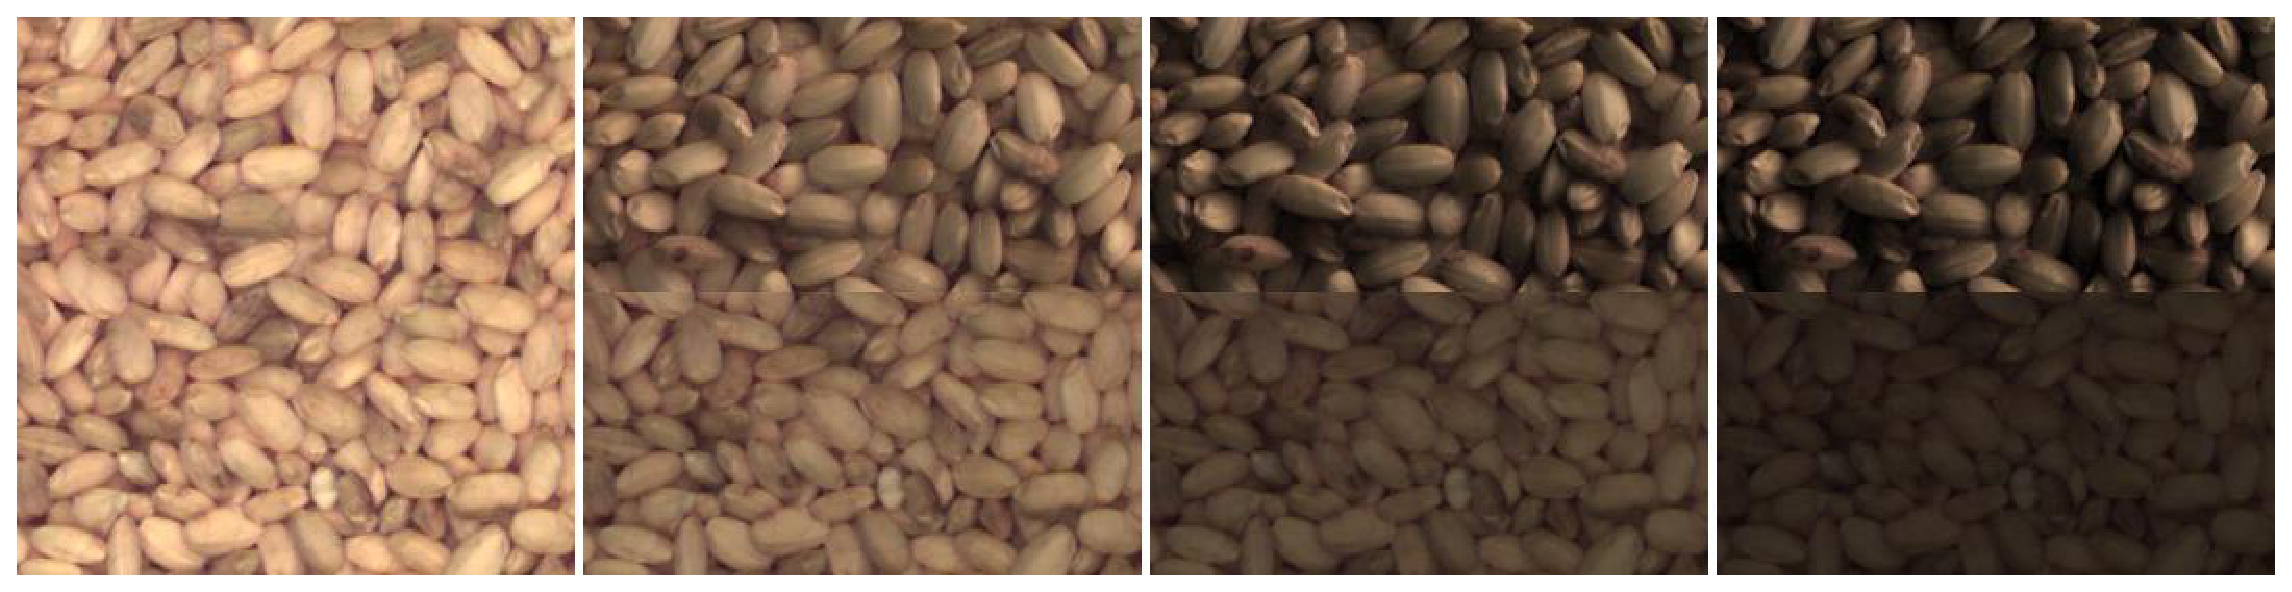
\includegraphics[scale=.4]{image_eps/ptm/ptm.eps}
\label{fig:subfig3} } \caption{PTM vs Conventional Texture Map: The upper portions of the images shows the visual appearance of
a PTM while the bottom half shows the conventional Texture map. Note how the former appears realistic while
the later suffers from unrealistic lighting and shadows.
} \label{fig:subfigureExample}
\end{figure*}
\end{center}
% The reflectance function of a scene point captures the appearance of that
% point as a function of lighting direction. We present an approach to printing
% the reflectance functions of an object or scene so that its appearance is
% modified correctly as a function of the lighting conditions when viewing the
% print. For example, such a “photograph��? of a statue printed with our approach
% appears to cast shadows to the right when the “photograph��? is illuminated
% from the left. Viewing the same print with lighting from the right will cause
% the statue’s shadows to be cast to the left. Beyond shadows, all effects
% due to the lighting variation, such as Lambertian shading, specularity, and
% inter-reflection can be reproduced. We achieve this ability by geometrically
% and photometrically controlling specular highlights on the surface of the
% print. For a particular viewpoint, arbitrary reflectance functions can be built
% up at each pixel by controlling only the specular highlights and avoiding
% significant diffuse reflections. Our initial binary prototype uses halftoning
% to approximate continuous grayscale reflectance functions.
% 
% An object’s appearance changes when lit from different directions.
% Shadows are cast and specular highlights shine. Even diffuse sur-
% faces change appearance, providing a valuable perceptual cue to ob-
% ject shape and material. Unfortunately, when printed on paper, this
% variability is lost. A photographic print represents just one appear-
% ance, regardless of the ambient lighting when the print is viewed.
% A real scene’s appearance at each point depends upon the in-
% cident illumination, the surface Bi-directional Reflectance Distri-
% bution Function (BRDF) [Nicodemus et al. 1977], and the local
% surface orientation. Typical printers cannot print images which re-
% act to incident illumination because they use inks with a limited
% range of BRDFs and print on paper which is flat, having a single
% orientation everywhere.
% Simply expanding the range of specularity of the printer’s inks is
% insufficient. Surface orientation plays an important role in control-
% ling the observed intensity of reflected light. To correctly represent
% this interaction with light, the local surface orientation of the paper
% needs to match that of the original object.
% A conceptually simple solution would be to orient the local sur-
% face normal of each pixel appropriately, and to print the object’s
% surface BRDF onto this pixel. However, this requires changing the
% physical shape of the underlying paper at the time of printing. This
% is an expensive process that requires equipment far more complex
% than just depositing ink onto a surface.
% We introduce a method of printing reflectance functions [Debevec
% et al. 2000] which makes use of paper with a static microgeometry
% structure, shown in Figure 1(b). The paper consists of a hexago-
% nal array of spherical depressions that have a specularly reflective
% surface. By selectively printing opaque or partially opaque ink on
% portions of that surface, we can control whether a specific inci-
% dent lighting direction returns a specular highlight, and to what
% degree. Because both the paper and ink are designed to minimize
% diffuse reflections, the specular return fully controls the appearance
% of this “reflectance paper��? and is used to control its appearance as a
% function of lighting direction. Note that this scheme gives sufficient
% expressive power to specify two dimensions of the 4D BRDF. We
% choose to specify, for a single fixed viewing direction, how much
% light will be reflected from each incident lighting direction, thereby
% building up an arbitrary reflectance function.
% The primary contribution of this work is a method for printing
% reflectance functions using existing printers and special paper. We
% support this contribution with a ray traced simulation and analysis
% of errors, as well as with an initial prototype implementation.
% 
% D reflectance functions can be measured easily for real scenes
% by taking photographs lit from many different lighting directions,
% and a wide variety of devices have been constructed to do so
% [Debevec et al. 2000; Malzbender et al. 2001; Peers et al. 2006;
% Wenger et al. 2005]. In principle this function can contain
% high-frequency components from specular highlights and hard
% shadows. However, in practice even low-order approximations are
% sufficient for a variety of presentation and evaluation purposes
% [Hawkins et al. 2001; Ramamoorthi et al. 2001]. Manipulations
% of reflectance functions have proved useful especially in both
% cinema applications [Debevec et al. 2000; Peers et al. 2007] and
% archeological applications [Freeth et al. 2006; Mudge et al. 2006].
% Figure 2 shows several examples of reflectance functions for in-
% dividual pixels, parameterized by the incoming illumination angle.
% 
% On the left is a set of colored leaves, with the reflectance of spe-
% cific marked pixels shown below. On the right are pixels chosen on
% opposite edges of almonds. Note that shadows are present in both
% cases at extreme lighting angles, and this shows up as dark regions
% in the reflectance function. Although the reflectance functions are
% very smooth, they are oriented differently at different pixels, and
% this is sufficient to provide a convincing perception of object shape
% when the incident light angle is changed. Flat paper printed with
% standard inks can only represent centered isotropic functions similar
% to the red pixel in this example. Our design can represent arbitrary
% functions. Note that for the photographically collected reflectance
% functions we employ, global illumination effects such as shadows
% and interreflections are present at the time of image capture, and thus
% are represented in the reflectance function. Whether such secondary
% effects are modeled is dependent on the generation of the reflectance
% data that is input to our system, whether captured or simulated.


\subsection{Polynomial Texture Maping}

Polynomial Texture Maps is a pixel based technique used to model luminiance
against changing lighting direction. 
It is an image-based technique that requires
no modeling of complex geometry. Only a set of images is required of the desired object to be used as a
texture which are taken from different known lighting
direction. 
PTMs reconstruct the color of a surface/texture under varying lighting
conditions. When a surface is rendered with a PTM, it takes on different illumination
characteristics depending on the direction of the light source.


PTM model uses a set of input images captured from a fixed camera, where each
image is illuminated from a specific known lighting direction. It uses a
biquadratic polynomial function with 6 coefficients per pixel for modeling the
reflectance. These coefficients are estimated from the set of input images(30 to
40), where the lighting direction is resolved into two components i.e
$l_{u}$,$l_{v}$ by projecting it on the image plane. These two components are
used as variables in the biquadratic function. Once the coefficients are
estimated fitting the model to the observed values, they are used to render
images from any given lighting direction.
The function used in PTMs is:

\begin{equation}
L(l_u,l_v) = al_u^2 + bl_v^2 + cl_ul_v + dl_u + el_v +f
\end{equation}

Polynomial Texture Mapping enables greatly improved realism
over conventional methods. Traditional texture mapping is used to
give the impression of geometric detail in a model using an image.
For example, a photograph of a brick wall may be used as a
texture map on a planar surface to avoid modeling the complex
surface detail of the brick. However, if the lighting in the
synthetic environment where the texture map is used is different
from the lighting the texture map was captured under, the
resulting rendering will appear incorrect and unrealistic. Worse
yet, when the texture is blended with the calculated lighting of a
geometric surface, the resulting rendering will look very flat and
smooth to the viewer.


But the PTM technique causes overall smoothening of light which dampens the effect
of specularity and softens sharp shadows. The effect of point light source is
reduced and the appearance is always similar to a diffused light source. Towards
this end, Drew {\em et al.} \cite{chap2-9} proposed modeling of shadows and
highlights in addition the the basic matt texture. The goal of this approach is
specifically to interpolate between two given images, and not a 3D texture model
of the surface.

We improve upon the PTM model to overcome the above limitations
and generate a complete 3D Texture model that can be evaluated at individual
pixels. We propose an approach to image-based lighting interpolation that is
based on estimates of geometry and shading from a set of input images. We
decompose images captured at different lighting conditions into intrinsic image
components; i.e, the {\em direct} and {\em global} image components. Each of
these components is then further separated to obtain different physical
phenomena such as shadows, specularity and luminance. A final image is obtained
by combining the the individual models together.

% To be written.
% PTM Representation
% Instead of representing light-dependent texture maps as a large number of source images, a compact 
% representation that can be rapidly evaluated is necessary. The representation used in Polynomial Texture Maps is 
% especially well suited for real-time games. For most materials other than mirrored surfaces the reflected light 
% varies smoothly as a function of incident light direction. This is because materials with rough microstructures 
% scatter light across a range of directions rather than a single reflected direction. As a result, in the illuminant
% domain the reflected light can be reproduced with low frequency representations. Any high-frequency effects that 
% do exist are blurred in light space and become smoother. Shadows cast by point light sources result in high 
% frequency changes in light space. Modeling with low frequency representations simply softens the hard shadows
% into what would be caused by area light sources. None of the softening in light space results in perceptually
% objectionable changes as it results in a plausible rendered appearance.
% Figure 2 shows two examples of PTMs 
% rendered from different illumination directions.
% The representation used in Polynomial Texture Maps is a biquadratic polynomial, which has sufficient degrees of 
% freedom to represent many different types of materials and objects while requiring a small number of parameters 
% per texel. 
% 
% L(u,v;l ,l ) a (u,v)l a (u,v)l a (u,v)l l a (u,v)l a (u,v)l a (u,v) u v u v 2 u v 3 u 4 v 5
% 
% The lu and lv input values are the projection of the desired incident light direction onto the texture coordinate system. 
% The PTM representation has six coefficients a0..a5 that 
% are fit to the captured source images for every texel. 
% Six scale and bias values are stored for each PTM to allow 
% the calculated coefficients to be stored at 8-bit precision while reproducing the range parameters. Typical 
% materials do not change their color significantly when the illumination direction is changed. For those materials, a 
% single polynomial per texel can be used to represent the texel luminance function. A separate normalized RGB 



% One of the advantages of this polynomial representation is that the output luminance depends linearly on the PTM 
% coefficients. This linearity means that applying mip-mapping and texture filtering directly on the coefficients 
% results in the correct appearance from the filtered coefficients. This is an improvement over bump mapping 
% techniques where naively filtering the bump map results in smoothing of the bump surface and incorrect 
% renderings. 
% When a luminance polynomial and RGB image is used for light-dependent texture mapping the storage 
% requirements are 6 8-bit coefficients and 3 8-bit color values per texel. While this is more data than standard 
% texture maps, this is much less data than the original source images that the PTMs reproduce. Compression 
% algorithms can be used to further reduce the size of the PTM. If compression is needed for offline storage than a 
% variant of JPEG can be used. By using JPEG compression on planes of coefficients for some of the coefficients, 
% and predicting other planes from the intracoded planes significant compression can be achieved with little 
% perceptual artifacts. For compression that can be processed by the GPU other techniques can be investigated. For
% example, vector quantization can be implemented directly on the GPU and should achieve good compression for 
% PTM datasets.
% The PTM technique is also useful for modeling other appearance effects that map well onto the polynomial 
% representation. For example, focus variation can be captured from photographs of a scene at multiple focus
% depths. The polynomial per texel then models the appearance of a pixel as a function of focal depth rather than
% light direction. The polynomial function can be reduced to a simpler 1D function as necessary depending on the 
% number of degrees of freedom. Other simple 1D and 2D effects that can be modeled with the low-frequency 
% representation can also be reproduced. High-frequency lighting such as specular highlights can also be rendered 
% by combining PTMs with existing rendering techniques. Most synthetic lighting models require the surface 
% normal for rendering. It is simple to estimate the surface normal for every texel of a PTM representing a diffuse 
% object. Since diffuse objects are brightest when the incident light direction aligns with the surface normal we can 
% solve for the light direction that maximizes the polynomial function to estimate the normal. During rendering the 
% PTM is evaluated as usual to recreate the captured material and then combined with the synthetic specular 
% reflectance.








% In a typical setup, a camera is mounted
% at the apex of a hemisphere of lights, and each light is then fired in turn, thus generating a
% sequence of images. Usually, some 40 to 50 images are used, with the larger the number of
% images the better.
% Thus PTM is a pixel-based method for modelling dependency of luminance (or RGB in a
% different embodiment) on lighting with the objective being relightable images. At each pixel,
% a 6-vector of coefficients is calculated using nonlinear least squares over the 2-vector of light-
% ing direction x, y-projected components. Subsequently, re-rendering can take place, e.g. by
% relighting images using a new lighting direction, by calculating surface normals and thence
% generating artificial specular highlights, by re-mapping colour, by increasing directional sen-
% sitivity to lighting direction in order to enhance contrast, by light source extrapolation, or by
% artificially varying focus


% Bump mapping [Blinn 78] is one proposed solution to this
% problem where the surface normals of underlying geometry are
% allowed to vary per texture element (texel). Introducing variations
% in the surface normals causes the lighting method to render the
% surface as though it had local surface variations instead of just a
% smooth surface. As a result, when the light is moved around the
% object, highlights appear due to the bump map and the surface
% appears to be rough, grooved or similarly modified as desired.
% Bump maps can be either hand modeled or, more typically,
% calculated procedurally. Creating a bump map to be used with real
% world textures from photographs is generally difficult. Methods
% have been developed that attempt to automatically generate bump
% maps from a set of input images under known light directions
% [Rushmeier 97]. These methods have difficulty with generating
% bump maps for objects with large surface variations that cause
% self-shadowing and intra-object interreflections. In addition,
% current bump map rendering techniques do not render shadows
% due to surface variation or brightened regions due to
% interreflections.


%The input light
%irections need not be uniformly spaced in the hemispherical set
% of possible light directions. We choose to represent the variation
% in surface color for each pixel independently with a simple
% biquadratic
% polynomial.
% Although
% approximate,
% this
% representation is compact and allows fast color reconstruction
% during rendering. One implementation of our method uses a
% polynomial to approximate the luminance of each texel, keeping
% the chromaticity constant. The result of our method is a texture
% map that properly reproduces the effects of variations in the
% illuminant direction relative to the object, whether due to the
% surface orientation of the texture-mapped object, or to changing of
% the location of the source. Intensity and color variations that are
% also due to self shadowing, sub-surface scattering and
% interreflections are also captured and modeled by PTMs. Figure 1
% compares our method to conventional texture mapping as lighting
% varies. Renderings using our method are very realistic, and require
% little or no user input once the input images are acquired.



\section{Text in Scene Images}

The aim of scene text localization and recognition is to find all areas in
an image that can be considered as text, mark
boundaries of the areas (rectangular bounding boxes) and output the word meanings of the detected content.
As the digital imaging devices are becoming cheaper and widely available, 
the size of the available digital image content is increasing rapidly.
The textual information present in images is very useful and needs to be extracted.
Therefore there is a growing demand to analyze, process and retrieve information
from multimedia content in an efficient way.
Some of the natural scene text images are shown in Fig \ref{}.

\begin{figure}[t]
\centering
\subfigure[]{
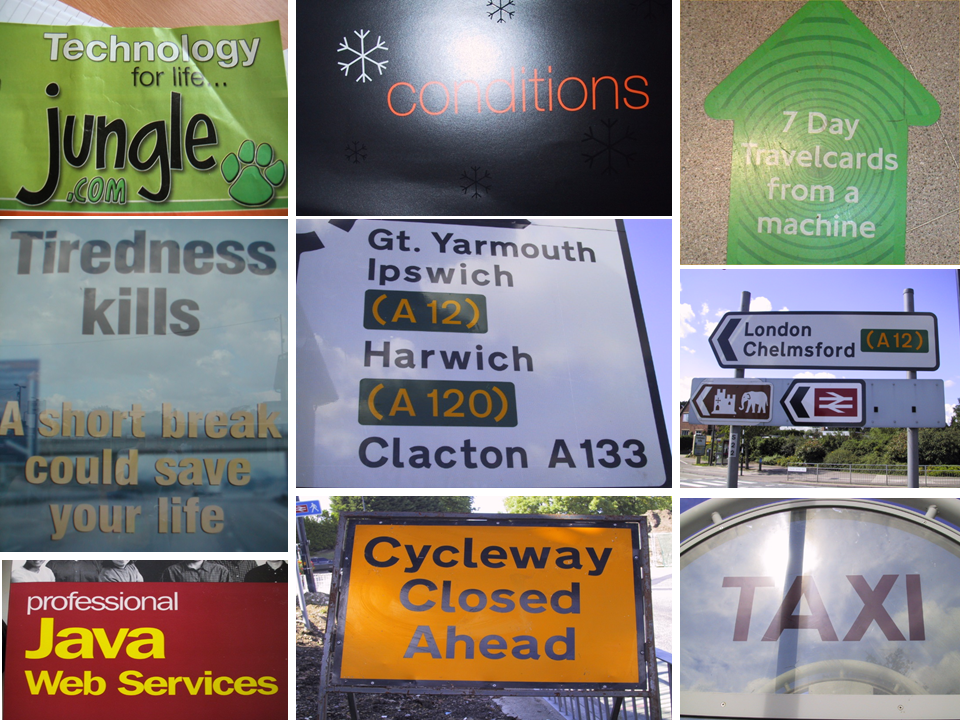
\includegraphics[height=4.3in,width=5.5in]{chap4/res_7/scene_images.eps}
}
\caption
{(a) Image containing Text over another Text (b) Foreground Text (c) Background Text (d)
Text extracted}
\end{figure}

\begin{figure}[t]
\centering
\subfigure[]{
\includegraphics[height=4.3in,width=5.5in]{chap4/res_7/text_pipe.eps}
}
\caption
{(a) Image containing Text over another Text (b) Foreground Text (c) Background Text (d)
Text extracted}
\end{figure}

Recognizing text in scene images is a challenging task.
This is because the quality and content of images are
rather unpredictable. There are many variations in backgrounds (non-uniform), textures,
fonts and lighting conditions that are present in images.
To build a full end-to-end text recognition system, we need to develop models
which are robust to these variations. They should read all the text within the image and extract information. 
 
Most of the work on scene text recognition tends to focus on a sub-component of the
full end-to-end text recognition system.
The general problem of end-to-end text recognition
consists of three primary components:  

\begin{itemize}
 \item \textbf{Text detection:} Is there any text and where is it in the image? Locate it.
\item \textbf{Text Segementation:} How to handle all the variations in background to extract 
foreground text as properly as possible.
\item \textbf{Text recognition:} What is the meaning of the word images?
\end{itemize}

In text
localization, the goal is to locate individual words or lines of text in the image.
The next step i.e text segmentation 
job is to extract the text properly so that it is better recognized afterwards. 
The extracted text goes to OCR for recognition.
Finally we identify the actual word meanings and
lines of the text. The recognized text is used in various applications. 
An example of the end-to-end recognition task is presented
in Fig \ref{}


\begin{figure}[t]
\centering
\subfigure{
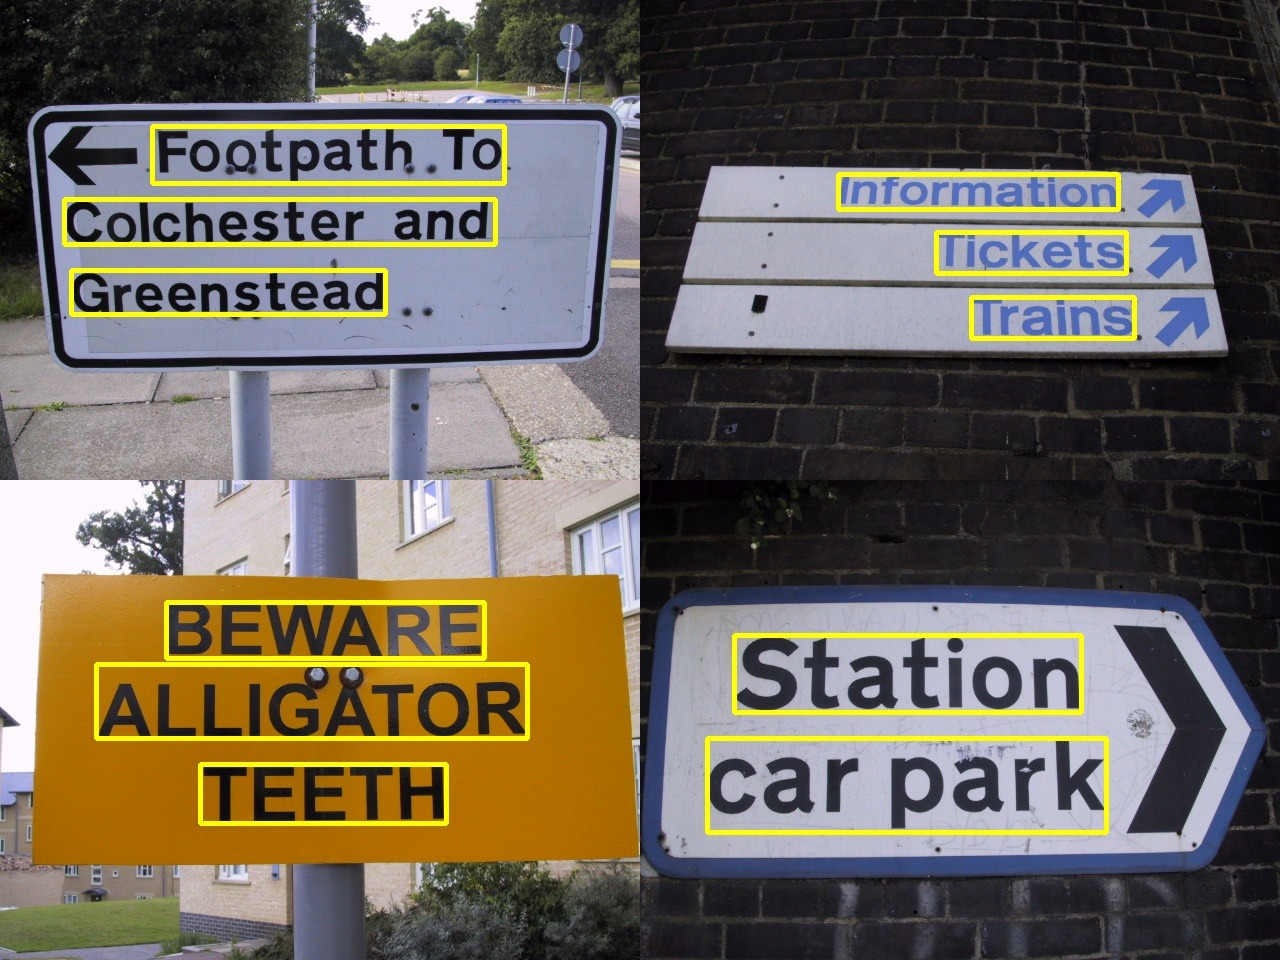
\includegraphics[height=4in,width=6in]{chap2/text_detect/results1.eps}
}
\caption
{(a) Image containing Text over another Text (b) Foreground Text (c) Background Text (d)
Text extracted}
\end{figure}


\begin{figure}[t]
\centering
\subfigure{
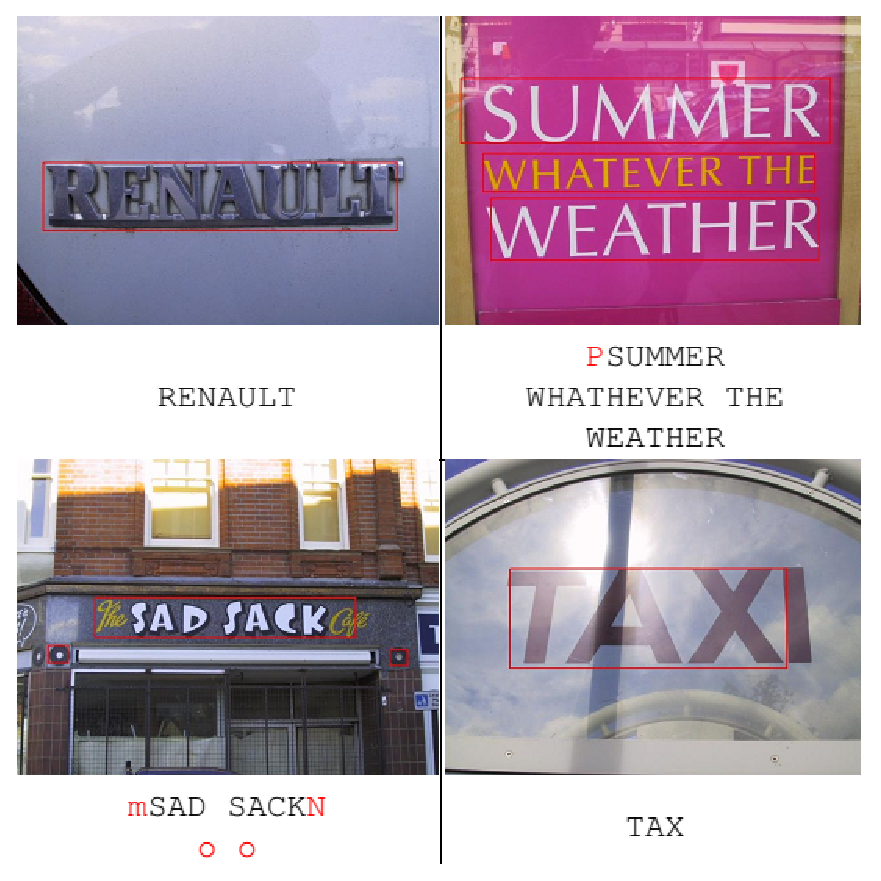
\includegraphics[height=3.6in,width=3in]{chap2/text_recog/res1.eps}
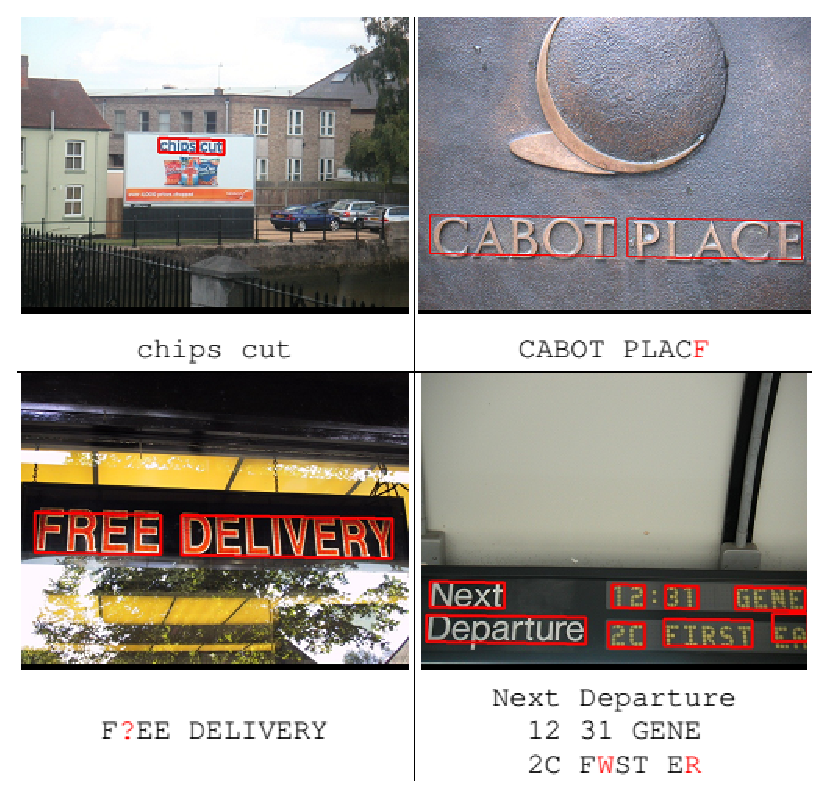
\includegraphics[height=3.6in,width=3in]{chap2/text_recog/res2.eps}
}
\caption
{(a) Image containing Text over another Text (b) Foreground Text (c) Background Text (d)
Text extracted}
\end{figure}


\subsection{Text Detection and Recognition}

As mentioned above, the goal of text detection or localization is to identify regions
of text in a given scene image. The task of detection is 
to identify rectangle bounding box for each word or each line of text in the image.
There are methods which focus on general text localization problem.
It can be categorized into
two groups - (a) methods based on a sliding window and (b) methods based
on grouping of regions. 
Methods in the first group \cite{chap2-1, chap2-2, chap2-3}[4, 18, 15]
use a texture-based approach for text detection. A window is moved over the whole image and the position of text is
estimated on the basis of local image features. 
These methods are also robust to noise.
But the computational complexity of these methods
is high because we need to search with many rectangles of different sizes and
aspect ratios. Also if the text is slanted or
perspectively distorted, then the sliding window methods do not produce
accurate text segmentation results.

Chen et al \cite{chap2-1}[4] uses AdaBoost classifier having intensity variance features, histogram features,
mean intensity features, derivative features and edge linking features. 
Then they use a variant of Niblack's adaptive binarization algorithm for segmentation. 
The method is
computationally expensive. It also
requires manual segmentation of many subwindows for training purposes and it seems
to over estimate the area of text in the image.
The above method was improved by Pan et. al \cite{chap2-2}[34] by adding a combination 
multi scale local binary battern and histogram of gradient
features in the text detection stage. A Markov Random Field
(MRF) is used to group segmented characters into words. The method claims better localization
performance but it still suffers from high computational complexity.
Recently, Lee et al. \cite{chap2-3} further improved the approach by adding
more computationally expensive features which slightly improved text localization performance
but it takes longer time for processing.
Lienhart et al \cite{chap2-4} uses a complex-valued multilayer feed-forward network 
which is trained to detect text at a fixed scale and position.
Coates et al \cite{chap2-5} used unsupervised machine learning techniques
for character detection and recognition. A 32x32 pixel window is
shifted over the entire image in multiple scales and each patch is classified using a
linear SVM classifier as text or non-text. A variant of K-means method is used 
to generate features during training which are then used by the classifier.
However, the method does not provide end-to-end text recognition.

Recently published methods are based on the second category i.e region grouping \cite{chap2-7, chap2-8, }.
[35, 10, 26, 47, 45, 25]. 
In these methods, certain local features are computed for each pixel in the image and
then pixels with similar feature values are grouped together using connected
component analysis to form characters. The methods can be scale-invariant and
they inherently provide character segmentation, which can be then used in an
OCR stage. The biggest drawback is a sensitivity to noisy and low-resolution
images, because they require low variance of local features in sufficient num-
ber of pixels.
Ohya et al [32] \cite{chap2-6} was the first method which was based on character localization. 
In their method, a local adaptive thresholding in grey-
scale images is used to detect candidate regions and regions with sufficient
contrast are selected as characters. Li et al. [16] apply thresholding in a
quantized color space and they group individual characters into text blocks
by simple alignment rules. Both methods assume that characters are upright
without any rotation, that the contrast is high and that background is uni-
form, which may be sufficient for signs or licence plates, but not for general
text localization.
Kim et al. [13] combine three independent detection channels (color con-
tinuity, edge detection and color variance) to find candidate regions. Can-
didate regions are grouped into blocks by size and position constraints and
each block is then divided into overlapping 16x16 pixel subblocks, which are
verified by a trained SVM classifier [7] using wavelet transform to generate
features. If a ratio of subblocks marked as text is higher than a predefined
threshold, the block is marked as text. The method is not scale-invariant be-
cause of the constant size of subblocks used for classification and the precision
is relatively bad because many small text-like patches are detected.
Takahashi and Nakajima [41] use a graph scheme, where vertices rep-
resent characters and edges represent a predecessor-successor relation in a
block of text. Candidate regions are found using Canny edge detector in the
CIELUV color space [5] and regions that pass a set of heuristic constraints
are considered vertices of the graph. Edges are created between neighboring
vertices and each edge is assigned a weight based on spatial distance, shape
and area similarity. Finally, a minimum spanning tree (MST) algorithm is
applied and edges with distance or angle over a predefined threshold are re-
moved. The method cannot handle illumination variations in foreground or
background and optimal edge weight estimation remains an open question.
Pan et al. [35, 36] create a text confidence map (see Figure 2) on a grey-
scale image pyramid using a calibrated Waldboost [40] classifier with His-
togram Of Gradient (HOG) features. Candidate regions are detected inde-
pendently on a grey-scale image using Niblack's binarization algorithm [31]
and a Conditional Random Field (CRF) [14] is employed to label regions as
text or non-text, considering the text condence as one of the unary features.
Then, a simple gradient graph energy minimization approach is applied to
form block of texts. The method is computationally expensive (because of
the image pyramid and the CRF inference) and its claimed localization per-
formance is questionable because a standard dataset was used [22], but with
a proprietary evaluation metric.
An image operator Stroke Width Transform (SWT) was introduced by
Epshtein et al. [10]. The SWT method finds edges using Canny detector [3]
and then estimates stroke width for each pixel in the image (see Figure 3).
Connected component algorithm is then applied to form pixels with similar
stroke width into character candidates, which are merged into text blocks
using several heuristic rules. The biggest limitation of the method is its de-
pendency on successful edge detection which is likely to fail on blurred or
low-contrast images. The method was further improved by Yao et al. [45]
where the heuristic rules for character candidate detection and text block
formation are replaced by trained classifiers with rotationally-invariant fea-
tures.




%The methods differ in their
%approach to individual character detection, which could be based on edge
%detection, character energy calculation or extremal region detection. While
%the methods are paying great attention to individual character detection,
%grouping of individual characters into words is performed based on heuristics
%or graph optimization methods and only unary and pairwise constraints are
%used.


All the methods listed above are focused solely on text localization, i.e.
they estimate position of the text, but do not provide its content. Our
method (first presented in [26]) was the first one to show end-to-end text
localization and recognition and only a few other methods that perform both
text localization and recognition have been published since. The method of
Wang et al. [42] nds individual characters as visual words using the sliding-
window approach and then uses a lexicon to group characters into words.
The method is able to cope with noisy data, but its generality is limited as
a lexicon of words (which contains at most 500 words in their experiments)
has to be supplied for each individual image.

2.1.1 Methods based on connected components analysis





% Detecting and reading text in scene images (also known
% as scene text localization and recognition or photo OCR)
% is an open problem of computer vision with many inter-
% esting applications, ranging from helping visually impaired
% people, translating language with an automatic input of text
% written in an unknown script, to indexing large image/video
% databases by their textual content (e.g. Google Street View,
% Flickr, etc.). Unlike traditional document OCR, none of the
% scene text recognition methods has yet achieved sufficient
% accuracy for practical applications (the winner of the most
% recent competition achieved a localization recall of only
% 62% [14]), which is why the problem has been recently re-
% ceiving significant attention.
% Text localization can be computationally very expensive
% because in an image of N pixels generally any of the 2N
% subsets can correspond to text. Text localization methods
% can be divided into two groups based on how they deal with
% this issue.
% The methods in the first group exploit a sliding-window

% approach to localize individual characters [17] or whole
% words [6], drawing inspiration from other object detection
% methods where this approach has been has been success-
% fully applied [2, 16]. Strengths of such methods include ro-
% bustness to noise and blur, because they exploit features ag-
% gregated over the whole region of interest. The main draw-
% back is that the number of rectangles that needs to be evalu-
% ated grows rapidly when text with different scale, aspect, ro-
% tation and other distortions has to be found - an effect which
% does not occur in general object detection tasks where the
% variance of sliding window parameters is lower.
% The second, recently more popular approach [4, 13, 11,
% 19, 12, 15] is based on localizing individual characters as
% connected components using local properties of an image
% (color, intensity, stroke-width, etc.). The complexity of the
% methods does not depend on the parameters of the text as
% characters of all scales and orientations can be detected in
% one pass and the connected component representation also
% provides character segmentation which can be exploited in
% an OCR stage. The biggest disadvantage of such methods
% is a dependence on the assumption that a character is a con-
% nected component, which is very brittle - a change in a sin-
% 
% gle image pixel introduced by noise can cause an unpro-
% portional change in the connected component size, shape or
% other properties, which subsequently affects its classifica-
% tion. The assumption also prevents the methods from de-
% tecting characters which consist of several connected com-
% ponents or where multiple characters are joint into a single
% connected component.
% 
% Several methods which focus only on a particular sub-
% problem (text localization [6, 13, 19, 4] or character respec-
% tively word cut-out recognition [3, 9]) have been published.
% Most relevantly, the method of Epstein et al. [4] converts an
% input image to a greyscale and uses the Canny detector [1]
% to find edges. Pairs of parallel edges are then used to cal-
% culate stroke width for each pixel and pixels with a similar
% stroke width are grouped together into characters. Along-
% side the aforementioned limitation of the connected compo-
% nents methods, the method also relies on a successful edge
% detection which might be problematic in noisy images and
% moreover it cannot handle ambiguities because each image
% pixel can belong to only one stroke. The proposed method
% differs radically from [4] in that it does not rely on hard de-
% cisions made by an edge detector, and in that it does not
% aim to estimate the stroke width (it actually assumes a unit
% stroke width - see Section 3.1), but rather it estimates the
% possible positions of strokes and detects characters based
% on known patterns of stroke orientations and their relative
% positions. The method of Epstein et al. provides character
% segmentation but does not perform text recognition.
% The method of Wang and Belongie [17] finds individ-
% ual characters as visual words using the sliding-window
% approach and then uses a lexicon to group characters into
% words. The method is able to cope with noisy data, but its
% generality is limited as a lexicon of words (which contains
% at most 500 words in their experiments) has to be supplied
% for each individual image and the sliding-window is limited
% to horizontal rectangles with a limited number of scales and
% aspects.
% An end-to-end text localization and recognition
% method [12] introduced by Neumann and Matas detects
% characters as a subset of Extremal Regions and then
% recognizes candidate regions in a separate OCR stage.
% The method performs well even on low contrast images
% and its computational complexity is close to real time.
% The text recognition however performs poorly on noisy
% images, because of the sensitivity induced by the connected
% component assumption. Moreover, the character represen-
% tation exploited in the method [11] is based on a direction
% of the boundary pixels chain-code, whose robustness is
% limited. For an exhaustive survey of text localization and
% recognition methods refer to the ICDAR Robust Reading
% competition results [8, 7, 14].
% 
% \subsection{Text Segmentation}
% 
% When the background is uneven as a result of poor or non-uniform lighting conditions, the image will not be 
% segmented correctly by a fixed gray-level threshold. These complex background vary dramatically depending on
% lighting, specularities, reflections and shadows.
%  The above methods applied directly to such images
% give poor results and cannot be used in OCR (Optical Character Recognition) systems. 
% 
% About OCR:
% Nowadays 
% OCR is considered a solved problem when a clean binarized and well formatted input image, with text in
% a standard font and language is provided. For instance, available OCR solutions, both commercial and
% open source, perform extremely well in documents generated with modern printers and standard font
% types. However, there are still some open research issues on OCR dealing with the recognition of rare
% font types or noisy copies and degraded documents, where one has to deal with dicult text segmentation, non
%  easily separable adjacent characters, or broken strokes. Furthermore, handwritten documents,
% colour-image document analysis, complex layouts and text segmentation in born-digital images are 
% examples of harder problems still unsolved and really hot topics for the Document Image Analysis community
% 
% Several methods for text binarization in natural images have
% been proposed more recently. For instance, Zhu et al. [7] suggested using the ordered 
% statistics filter for estimating thresholds in the non-linear Nilblack decomposition. Howe [12]
% proposed to use the Laplacian of the image intensity for
% scanned document binarization within a Markov Random Field
% model (which is an algorithmic setup most similar to the one
% we propose below). Gatos et al. [13] used two binarized images by Sauvola’s method for original gray-scale and inverted
% images for rough estimation of background and thresholded
% the difference between original and binarized images. Ezaki
% et al. [14] proposed generating connected components by
% combination of mathematical morphology operations, edge
% extraction and Otsu thresholding of image color channels.
% Epshtein [15] suggested using a new image operator (Stroke
% Width Transform) to segment letters. Minetto et al. [16]
% proposed using toggle mapping for character segmentation in
% a multiresolutional way since natural scene images have large
% character size variations and strong background clutter.
% 
% Mishra {\em et al}~\cite{A16} has recently formulated the problem of binarization as an MRF optimization problem. 
% The method shows superior performance over traditional binarization methods on many images, and we use it as the
% basis for our comparisons. However, their method is sensitive to the initial auto seeding process.
